
\section{Schwachstelle 12: Mutmaßlicher Innentäter ausgehend von Host Esperanza}
\label{sec:vuln12}
Eine auffällige verschlüsselte Datei \texttt{HackingNotizen.txt} im Ordner \texttt{Eigene Dokumente} des Benutzers \texttt{Lightman} auf dem Host \texttt{Esperanza} lässt mutmaßlich auf einen Innentäter schließen. Die in der Text-Datei beschriebenen Aktionen dokumentieren die mutmaßliche Vorgehensweise des Angreifers und stimmen mit den in diesem Penetration-Test gefundenen Schwachstellen überein.


\subsection{Beschreibung der Schwachstelle}
\label{subsec:vuln12_way}


Abbildung \ref{fig:vuln11_docs_encrypted} zeigt, dass der Inhalt des Ordners \texttt{Eigene Dokumente} des Benutzers \texttt{Lightman} mit den Betriebssystemmittel von Windows verschlüsselt ist und daher nur geöffnet werden kann, sofern der Benutzer \texttt{Lightman} mit dem zum Konto dazugehörigen Passwort angemeldet ist. SYSTEM-Berechtigungen, welche aus der zuvor beschriebenen Bluekeep-Schwachstelle erlangt werden können, können diesen Verschlüsselungsschutz somit nicht umgehen.


\begin{figure}[h]
    \centering
    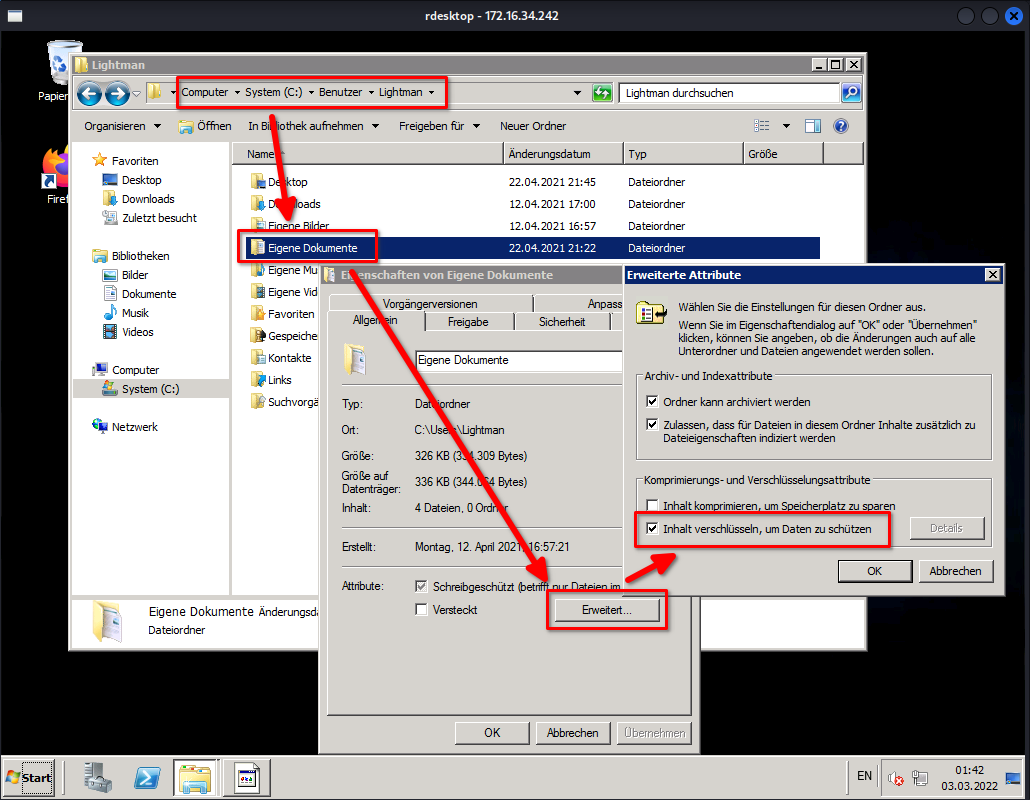
\includegraphics[width=\textwidth]{./img/vuln11_inside/docs_encrypted}
    \caption{Verschlüsselte \texttt{Eigene Dokumente} des Benutzers \texttt{Lightman} auf \texttt{Esperanza}}.
    \label{fig:vuln11_docs_encrypted}
\end{figure}



Innerhalb des \texttt{Eigene Dokumente}-Ordners sind 3 Dateien abgelegt, die in Abbildung \ref{docs_content} dargestellt werden.


\begin{figure}[h]
    \centering
    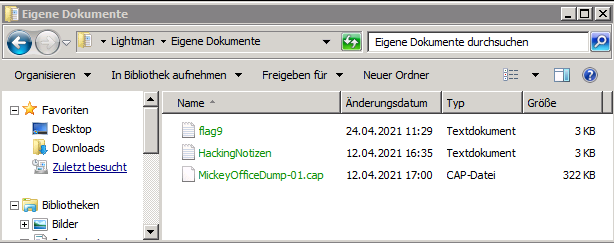
\includegraphics[width=0.7\textwidth]{./img/vuln11_inside/docs_content}
    \caption{Inhalt von \texttt{Eigene Dokumente} des Benutzers \texttt{Lightman} auf \texttt{Esperanza}}.
    \label{docs_content}
\end{figure}

Zur Ermittlung der SHA256-Hashwerte der Dateien wurden diese kurzfristig auf den Desktop des Benutzers \texttt{Lightman} kopiert und der Verschlüsselungsschutz aufgehoben (s. Abbildung \ref{encryption_removed}) , um die Dateien anschließend über die bestehende Meterpreter-Sitzung mit \texttt{SYSTEM}-Berechtigungen herunterzuladen (s. Abbildung \ref{sha256sum}).




\begin{figure}[h]
    \centering
    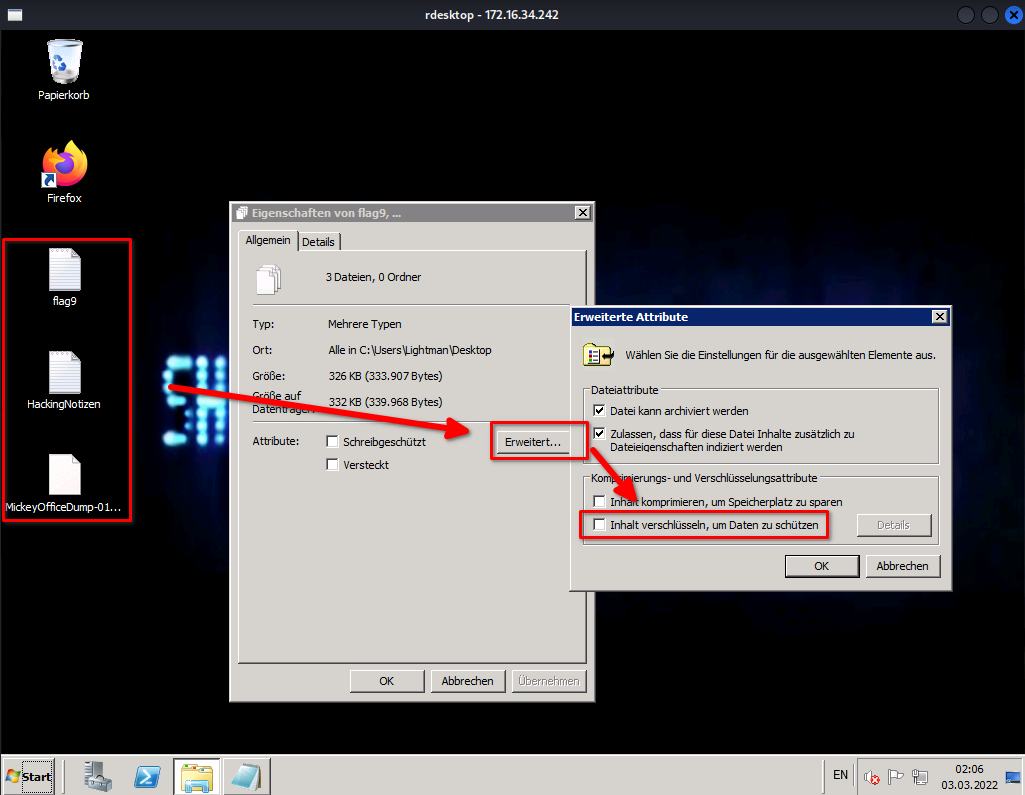
\includegraphics[width=\textwidth]{./img/vuln11_inside/encryption_removed}
    \caption{Kopieren der Dokumente auf den Desktop und entfernen der Verschlüsselung.}
    \label{encryption_removed}
\end{figure}



\begin{figure}[h]
    \centering
    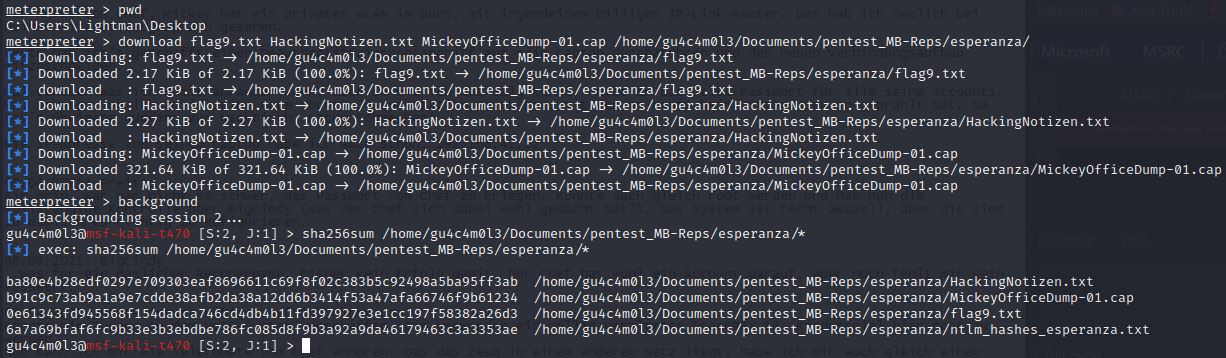
\includegraphics[width=\textwidth]{./img/vuln11_inside/sha256sum}
    \caption{Herunterladen und bilden der SHA265-Prüfsumme der Dateien innerhalb von \texttt{Eigene Dokumente}.}
    \label{sha256sum}
\end{figure}

Abbildung \ref{flag9_content} legt den Inhalt der Datei \texttt{flag9.txt} dar und Abbildung \ref{hackingnote_content} zeigt den Inhalt der Datei \texttt{HackingNotizen.txt}.

\begin{figure}[h]
    \centering
    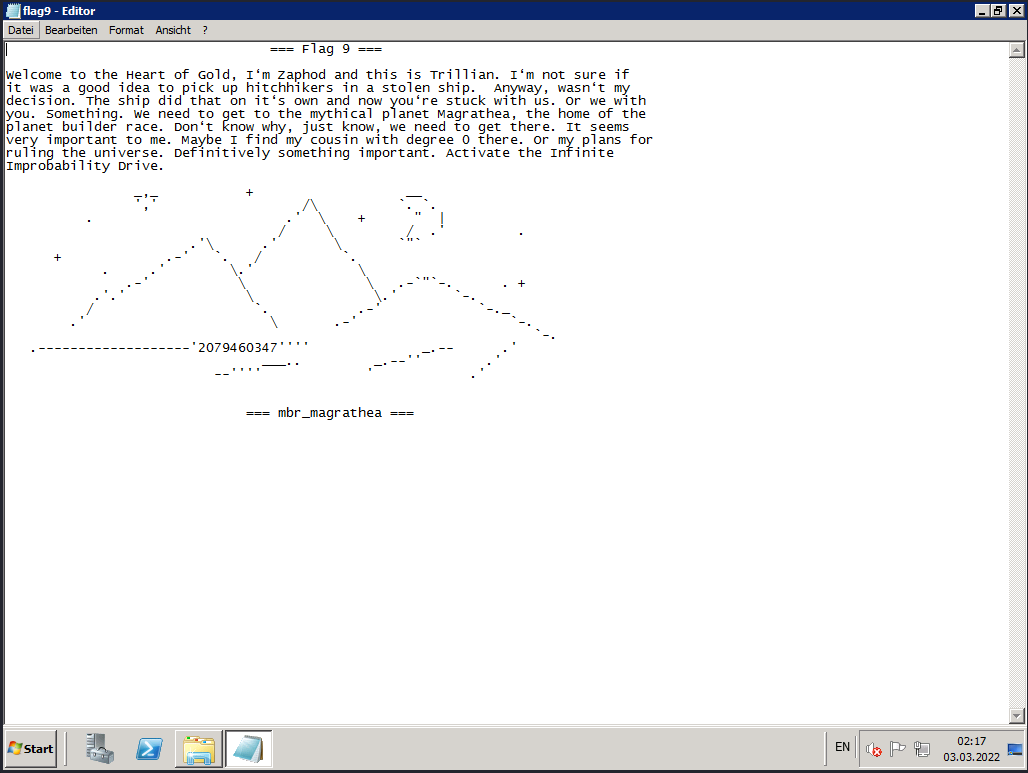
\includegraphics[width=\textwidth]{./img/vuln11_inside/flag9_content}
    \caption{Inhalt der Datei \texttt{flag9.txt}.}
    \label{flag9_content}
\end{figure}

\begin{figure}[h]
    \centering
    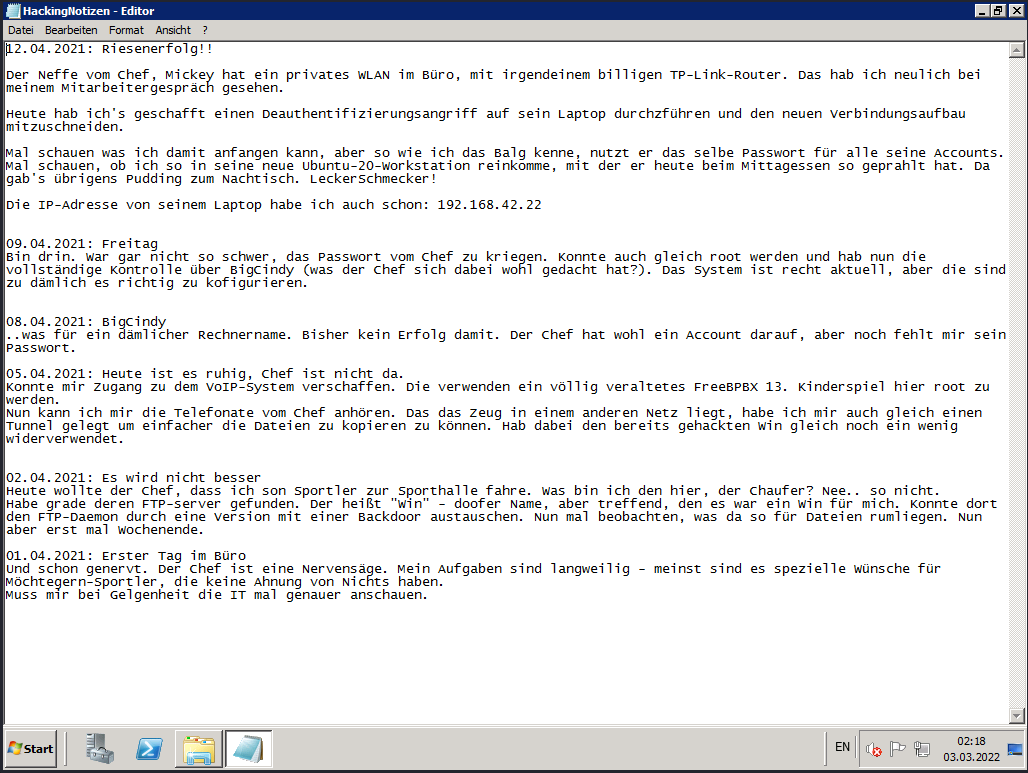
\includegraphics[width=\textwidth]{./img/vuln11_inside/hackingnote_content}
    \caption{Inhalt der Datei \texttt{HackingNotizen.txt}.}
    \label{hackingnote_content}
\end{figure}

Insbesondere der Inhalt der Datei \texttt{HackingNotizen.txt} lassen mutmaßen, dass ausgehend vom Benutzerkonto \texttt{Lightman} auf dem Host \texttt{Esperanza} Angriffe auf die interne Infrastruktur durchgeführt wurden. So scheint am 02.04.2021 die auf dem Host \texttt{win} aufgedeckte vulnerable ProFTPD-Software mutmaßlich durch eine Version mit eingebauter Backdoor ausgetauscht worden zu sein. Darüber hinaus wurde mutmaßlich am 05.04.2021 über die in Kapitel \ref{sec:vuln5} vorgestellten Schwachstelle das FreePBX-System mit Root-Rechten kompromittiert und eine Tunnel-Verbindung zum Host \texttt{win} aufgebaut. Des Weiteren wurde mutmaßlich am 08.04.2021 das Passwort des Benutzers \texttt{myron} gebrochen und somit Zugriff auf das System \texttt{BigCindy} erlangt. Abschließend konnte aus der Textdatei entnommen werden, dass am 12.04.2021 mutmaßlich das WLAN-Passwort vom Neffen des CEOs, Mickey Bolitar, gebrochen wurde und anschließend mit dem gleichen Passwort auf den Host \texttt{Mickey} angemeldet werden konnte. Zu dem in der Textdatei genannten Aktionen konnten keine belegenden Beweise gefunden werden. Allerdings stimmen die detaillierten Angaben innerhalb der Textdatei mit den gefundenen Schwachstellen während des Penetration-Tests überein. Daher wird aufgrund der Faktenlage ein mutmaßlicher Innentäter ausgehend vom Benutzerkonto \texttt{Lightman} auf dem Host \texttt{Esperanza} vermutet.

Die Analyse des Netzwerkmitschnitts der Datei \texttt{MickeyOfficeDump-01.cap} wird im nachfolgenden Kapitel vorgestellt.


\subsection{Risikobewertung}
Die Korrektheit und der Detailgrad der in der Textdatei \texttt{HackingNotizen.txt} gefundenen Informationen geben Grund zur Annahme, dass ein potenzieller Innentäter mit weitreichenden IT-Kenntnissen ausgehend vom Benutzerkonto \texttt{Lightman} auf dem Host \texttt{Esperanza} Angriffe auf verschiedene Hosts innerhalb der Firmen-Infrastruktur ausgeführt hat. Die Eintrittswahrscheinlichkeit und die Schadenshöhe wurde daher mit HOCH bewertet.

Das Gesamtrisiko wurde abschließend mit \textcolor{red}{HOCH} eingeschätzt.

\subsection{Empfohlene Gegenmaßnahmen}
Es wird empfohlen ein Incident-Response-Team forensische Ermittlungen über die in der Datei \texttt{HackingNotizen.txt} dargelegten Informationen zu beauftragen. Darüber hinaus sollte die Person, welche das Benutzerkonto \texttt{Lightman} auf dem Host \texttt{Esperanza} zu den Inhalten der Textdatei befragt werden und das Alibi zu den dokumentierten Zeitpunkten geprüft werden.

\subsection{Hinterlassene Spuren und Spurenbeseitigung}
Es wurden keine Dateien geändert, hinzugefügt oder Prozesse gestartet.


